

%\documentclass[journal,10pt,draftclsnofoot,onecolumn]{IEEEtran} %draftclsnofoot
%\documentclass[confl, draftclsnofoot]{IEEEtran}
%\documentclass[conference,onecolumn,draft]{IEEEtran}
\documentclass[conference]{IEEEtran}
\usepackage{grffile}
\usepackage{color}
\usepackage{graphicx}
\usepackage{cite}
\usepackage{multicol}
\usepackage{subcaption}
\usepackage{algorithm}
\usepackage{algpseudocode}
\usepackage{pifont}
\usepackage{subcaption}
\usepackage{siunitx}

%\usepackage{setspace}
%\doublespacing
%\onecolumn
\begin{document}
%
% paper title
% can use linebreaks \\ within to get better formatting as desired
\title{Bridging the Multiscale gap: Identifying Cellular Parameters from Multicellular Data\\}
%
%
% author names and IEEE memberships
% note positions of commas and nonbreaking spaces ( ~ ) LaTeX will not break
% a structure at a ~ so this keeps an author's name from being broken across
% two lines.
% use \thanks{} to gain access to the first footnote area
% a separate \thanks must be used for each paragraph as LaTeX2e's \thanks
% was not built to handle multiple paragraphs
%




\author{Qanita~Bani Baker, Gregory~J.~Podgorski, Christopher D. Johnson, Elizabeth Vargis, Nicholas~S.~Flann % <-this % stops a space
\IEEEcompsocitemizethanks{Qanita~Bani Baker, Gregory J. Podgorski, Elizabeth Vargis, and ~Nicholas~S.~Flann  are with Utah State University, Logan, Utah,  USA.
e-mail: (qanita@aggiemail.usu.edu, gregory.podgorski@usu.edu, christopher.d.johnson@aggiemail.usu.edu, elizabeth.vargis@usu.edu, and nick.flann@usu.edu)}}% <-this % stops a space


% note the % following the last \IEEEmembership and also \thanks -
% these prevent an unwanted space from occurring between the last author name
% and the end of the author line. i.e., if you had this:
%
% \author{....lastname \thanks{...} \thanks{...} }
%                     ^------------^------------^----Do not want these spaces!
%
% a space would be appended to the last name and could cause every name on that
% line to be shifted left slightly. This is one of those "LaTeX things". For
% instance, "\textbf{A} \textbf{B}" will typeset as "A B" not "AB". To get
% "AB" then you have to do: "\textbf{A}\textbf{B}"
% \thanks is no different in this regard, so shield the last } of each \thanks
% that ends a line with a % and do not let a space in before the next \thanks.
% Spaces after \IEEEmembership other than the last one are OK (and needed) as
% you are supposed to have spaces between the names. For what it is worth,
% this is a minor point as most people would not even notice if the said evil
% space somehow managed to creep in.



% The paper headers
%\markboth{Journal of \LaTeX\ Class Files,~Vol.~6, No.~1, January~2007}%
%{Shell \MakeLowercase{\textit{et al.}}: Bare Demo of IEEEtran.cls for Journals}
% The only time the second header will appear is for the odd numbered pages
% after the title page when using the twoside option.
%
% *** Note that you probably will NOT want to include the author's ***
% *** name in the headers of peer review papers.                   ***
% You can use \ifCLASSOPTIONpeerreview for conditional compilation here if
% you desire.




% If you want to put a publisher's ID mark on the page you can do it like
% this:
%\IEEEpubid{0000--0000/00\$00.00~\copyright~2007 IEEE}
% Remember, if you use this you must call \IEEEpubidadjcol in the second
% column for its text to clear the IEEEpubid mark.



% use for special paper notices
%\IEEEspecialpapernotice{(Invited Paper)}




% make the title area
\maketitle

\begin{abstract}
Put our abstract here.

\end{abstract}


% IEEEtran.cls defaults to using nonbold math in the Abstract.
% This preserves the distinction between vectors and scalars. However,
% if the journal you are submitting to favors bold math in the abstract,
% then you can use LaTeX's standard command \boldmath at the very start
% of the abstract to achieve this. Many IEEE journals frown on math
% in the abstract anyway.

% Note that keywords are not normally used for peerreview papers.
\renewcommand\IEEEkeywordsname{Key Words}
\begin{IEEEkeywords}
Systems Biology, Agent-Based Model, Parameter Estimation, Optimization, Micropatterning, Vascular endothelial growth factor (VEGF).
\end{IEEEkeywords}








% For peer review papers, you can put extra information on the cover
% page as needed:
% \ifCLASSOPTIONpeerreview
% \begin{center} \bfseries EDICS Category: 3-BBND \end{center}
% \fi
%
% For peerreview papers, this IEEEtran command inserts a page break and
% creates the second title. It will be ignored for other modes.
%\IEEEpeerreviewmaketitle



\section{INTRODUCTION}
\IEEEPARstart


An important aspect of computational systems biology is the investigation of dynamic biological processes that operate across multiple temporal and spatial scales by constructing and running multiscale models \cite{Kang2014Biocellion}, \cite{qanitabaker:Materi2007Computational}, \cite{qanitabaker:DiazOchoa2012Multiscale}, \cite{qanitabaker:Castiglione2014Modeling}, \cite{Vicini2010Multiscale}. These models incorporate a set of parameters that represent the physical and chemical properties of the biological system \cite{qanitabaker:Mahoney2012Multiobjective}. The parameters are used to define the components of the models that when simulated reproduce the behavior of the biological system. Often the correct values of these parameters are unknown or difficult to obtain \cite{qanitabaker:Walker2007Challenges}, \cite{qanitabaker:Transtrum2009Why}.

Recently, there has been an increase in the number of model-fitting methods proposed to estimate model parameters' values \cite{qanitabaker:RodriguezFernandez2006Novel}, \cite{qanitabaker:Chou2009Recent}, \cite{qanitabaker:Sun2012Parameter} from experimental data.  Without accurate estimations of parameters, predictions from simulation studies will most likely be erroneous and provide little scientific insight and guidance in disease treatment  \cite{qanitabaker:Banga2008Optimization}. This scenario can be ameliorated by fitting the model to experimental \textit{in vitro} / \textit{in vivo} data \cite{qanitabaker:BalsaCanto2008Hybrid} \cite{qanitabaker:Lillacci2010Parameter}. Finding the best-fit values for the unknown parameters enhances the possibility of performing accurate quantitative predictions.

 Vascular endothelial growth factor (VEGF) is a key promoter of angiogenesis and vascular development and is the target in numerous anti-angiogenic therapies \cite{Carmeliet2000Angiogenesis}. Angiogenesis is the growth of blood vessels from the preexisting vasculature, a process involved in the physiological functions of several diseases, such as cancer and age-related macular degeneration (AMD). Moreover, in spite of substantial basic science and translational research to develop anti-angiogenic therapies, many questions remain about the mechanisms of action of angiogenic drugs, how and why several diseases such as AMD become resistant to the treatment, or the patient conditions that can benefit most from these drugs \cite{Bergers2008Modes}. For these reasons, computational models of angiogenesis have been developed to simulate the process and provide a framework for generating and testing hypotheses of VEGF-driven processes \cite{qanitabaker:MacGabhann2006Computational, qanitabaker:Stefanini2008Compartment, qanitabaker:Gabhann2012Simulating}. Models have aided in the development of novel and effective anti-angiogenic therapeutics that target VEGF regulation and receptors \cite{qanitabaker:Mahoney2012Multiobjective}, \cite{qanitabaker:Finley2013Compartment,qanitabaker:Yen2011TwoCompartment}. Advancing these computational approaches combined with progress in \textit{in vitro} experimental studies will shed light on these issues by providing an effective framework for generating and testing hypotheses related to VEGF regulation and transport in the tissue \cite{qanitabaker:Stefanini2008Compartment}.

 An essential mechanism for understanding VEGF's role in disease development is its auto-regulation. The rate of VEGF secretion is controlled through an auto-inhibitory regulatory mechanism where the VEGF concentration of a cell's microenvironment down-regulates the secretion of VEGF. This control loop enables a community of cells to maintain a stable background concentration of VEGF \cite{Takahashi2005Vascular}. Disruption of the loop is implicated in multiple disease states.

 This paper presents a method for accurately characterizing this auto-regulation, not from microfluidic assays that interrogate individual or mixed cell populations but from spatially organized multicellular experimental data sampled over time. As will be explained later, spatiotemporal data provides unique insights because auto-regulation is inherently a mechanism that is manifested over space and time. The rest of the paper is structured as follows: First the experimental setup and computational model is described, along with the specific autoregulatory parameters that are known and those to be estimated. Second, the search method for finding the values for the parameters is described in detail. Next the method is evaluated by validating the identified parameter values. Finally, a summary of the method's effectiveness and suggestions for future work are given.

\section{Multicellular Experiment and Model}

Describe the study here.





% The very first letter is a 2 line initial drop letter followed
% by the rest of the first word in caps.
%
% form to use if the first word consists of a single letter:
% \IEEEPARstart{A}{demo} file is ....
%
% form to use if you need the single drop letter followed by
% normal text (unknown if ever used by IEEE):
% \IEEEPARstart{A}{}demo file is ....
%
% Some journals put the first two words in caps:
% \IEEEPARstart{T}{his demo} file is ....
%
% Here we have the typical use of a "T" for an initial drop letter
% and "HIS" in caps to complete the first word.



\section{METHOD}

Explain the research method here.  How did we study the problem?




\section{RESULTS}

Building upon Davis et al, a two dimensional factory was used in this work. The height of the factory was set to 0.768 mm while the width was fixed at 1.536 mm. The total number of producer and vascular cells were 4200 and 1800, respectively where vascular cells contributed to 30 per cent of total number of cells. A total of 384 circulatory cells simulating the external delivery and product extraction system existed as two identical columns on two sides of the factory. The number of all mentioned cells were kept constant through the experiment. The simulations started with a random distribution of producer and vascular cells inside the factory. After 16 simulation hours, the factory started the production phase provided the existence of a network of vascular cells. The aggregate product amount collected by the vascular network and circulatory columns was output after 2 simulated hours as the final throughput of the system. 
\\
\\
A genetic algorithm with a population of 3 chromosomes over an evolution of 500 steps was used for obtaining the optimal values for the seven mentioned parameters. 
\\
\\
Figure 1 shows the throughput of our cell factory during the evolution of this genetic algorithm. After 500 sweep iterations, the highest total product of the factory reached 616.65788 ug. The parameter values contributing to the best case are shown in Table 1. The factory related to these parameters is depicted in figure 2. 

\begin{figure}[!t]
\centering
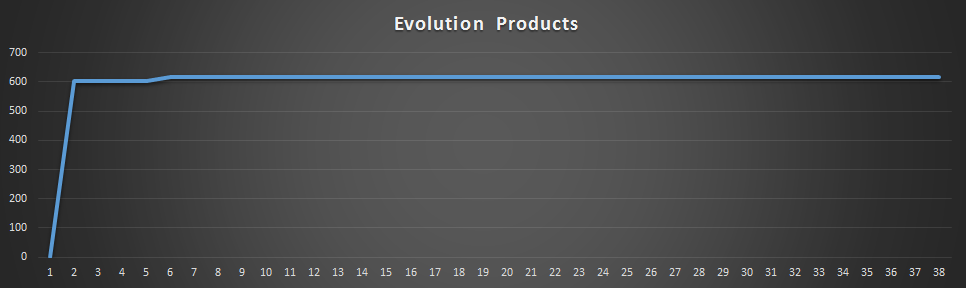
\includegraphics[width=3in]{./figures/sima/results/evolution products.png}

\caption{The amount of product values $Product$ with evolution number $It$}
\label{product}
\end{figure}          

\begin{table}[!t]
\renewcommand{\arraystretch}{1.3}
\caption{The best parameter values the genetic algorithm has identified}
\label{parameter_table}
\centering
\begin{tabular}{c||c}
\hline
\bfseries Parameter & \bfseries Value\\
\hline\hline
\\
\hline
Chemotactic Strength With Gradient & 2.34110242590437\\
\hline
Vascular Cells' Production Rate & 6.1583863371631\\
\hline
Circulatory Cells' Production Rate & 4.26190176330675\\
\hline
Vascular Cells' Chemo-attractant Decay Rate & 0.00839922309567474\\
\hline
Circulatory Cells' Chemo-attractant Decay Rate & 0.0000282503099488372\\
\hline
Vascular Cells' Half-saturation Rate & 0.0092723921166939\\
\hline
\end{tabular}
\end{table}

\begin{figure}[!t]
\centering
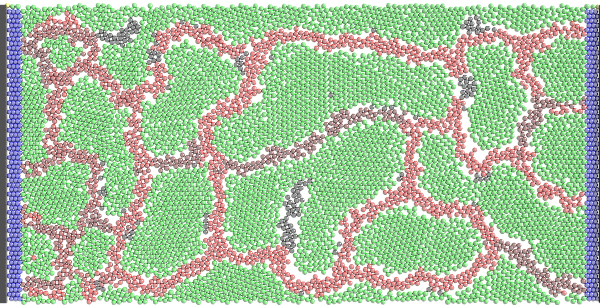
\includegraphics[width=3in]{./figures/sima/results/highest product factory.png}

\caption{The factory with the highest throughput which was found by the GA}
\label{factory}
\end{figure}   





%\section{SUMMARY}

\section{CONCLUSION}


Wrap up the conclusions here.



%%//Future works  In this model error minimization is used to determine model parameters that optimally fit the data are. The best model parameters should be found by choosing, among suboptimal parameters, those that match criteria other than the ones used to fit the model \cite{qanitabaker:Slezak2010When}. In the %future, other biological criteria need to be addressed in finding data and optimization approach form a new complex system and point to the need of a theory that addresses this problem more generally.
% use section* for acknowledgement
\section*{Acknowledgment}

This work was supported by the Luxembourg Centre for Systems Biomedicine, the University of Luxembourg and the Institute for Systems Biology, Seattle, USA. Research reported in this publication was partially supported by the National Institute Of General Medical Sciences of the National Institutes of Health under Award Number P50GM076547. The content is solely the responsibility of the authors and does not necessarily represent the official views of the National Institutes of Health.


\bibliographystyle{plain}

\begin{small}

\bibliography{qanitabaker-retinal,qanitabaker-fittingthree,nicholasflann}


\end{small}







\end{document}


